
%PREAMBLE
%%%%%%%%%%%%%%%%%%%%%%%%%%%%%%%%%%%%%%%%%%%%%%%%%%%%%%%

\documentclass[titlepage,norsk,a4paper,10pt]{article}
\usepackage{babel,graphicx}
\usepackage[utf8]{inputenc}
%\usepackage{listings}

\title{Assignment 4 IT3708}
\author{Odd Andreas Sørsæther \and Andreas Hagen}

%\lstset{frame=tb,
%  language=C,
%  aboveskip=3mm,
%  belowskip=3mm,
%  showstringspaces=false,
%  columns=flexible,
%  basicstyle={\small\ttfamily},
%  numbers=none,
%  numberstyle=\tiny\color{gray},
%  keywordstyle=\color{blue},
%  commentstyle=\color{dkgreen},
%  stringstyle=\color{mauve},
%  breaklines=true,
%  breakatwhitespace=true
%  tabsize=3
%}

%%%%%%%%%%%%%%%%%%%%%%%%%%%%%%%%%%%%%%%%%%%%%%%%%%%%%%%

\begin{document}
\maketitle


\section{Description of implementation}


The system consists of four C-classes, the provided classes stagnation, search and retrieval and the controller class swarm\_controller. The swarm\_controller class includes the three provided classes and has only one method, the main method. The main method reads the sensor values from the robot, feeds them to the layers and activates the actuators based on the subsumption architecture where the higher levels subsume the lower levels. In practice, this means that the search layer is set as the default layer and if nothing else happens, the wheel speed computed by the search layer is used. If the retrieval layer receives more input than a given threshold from the front IR\-sensors, the retrievel layer returns wheel speeds, and the wheel speeds provided by the retrieval layer is used. Finally, if the stagnation layer returns wheel speeds, those wheel speeds are used.

The  first part of the while-loop reads sensor data using the following lines of code:


\begin{verbatim}
for(i=0; i<8; i++){
	distance_sensors[i] = wb_distance_sensor_get_value(ps[i]);
	}

for (i=0; i<8 ; i++){
       light_sensors[i] = wb_light_sensor_get_value(ls[i]);
    }

\end{verbatim}

The wheel speeds from the search layer are then collected by calling:

\begin{verbatim}
update_search_speed(distance_sensors, SEARCH_THRESH);
search_left_wheel_speed = get_search_left_wheel_speed();
search_right_wheel_speed = get_search_right_wheel_speed();

\end{verbatim}


The swarm\_retrieval method activates the retrieval layer which will calculate actuator commands based on the sensory input. The method returns a boolean int that is true if the retrieval layer decides that one or more of the IR sensors  are high enough for it to investigate. If this is true, the control is submitted to the retrieval layer. 

\begin{verbatim}

int senses_something = swarm_retrieval(light_sensors, RETRIEVAL_THRESH);   

    if(senses_something){
        CONTROLLING_LAYER = RETRIEVAL_LAYER;
    }
  
if(stagnation == 0 && distance_sensors[7] > 300){ 
        EPOCH_TIME = EPOCH_TIME+1;

       if(EPOCH_TIME > 150){ 
          EPOCH_TIME = 0;
          reset_stagnation();
          valuate_pushing(distance_sensors,previous_distance_sensors);
       }
    }



\end{verbatim}

Internally, the stagnation checks if it is in stagnation and decides upon an action accordingly. It the returns a boolean int and if this int is 1 (true) then the control is submitted to the stagnation layer.

\begin{verbatim}
stagnation = stagnation(distance_sensors, DIST_THRESHOLD);
	
	if(stagnation){
		CONTROLLING_LAYER=STAGNATION_LAYER;
	}
	
	stagnation_left_wheel_speed = get_stagnation_left_wheel_speed();
	stagnation_right_wheel_speed = get_stagnation_right_wheel_speed();

\end{verbatim}

Robots never went into stagnation-mode while pushing the box, later discovered that this was due to how valuate\_pushing() is implemented and changed it slightly

\section{Expected and unexpected behaviours}

Expectedly, the robots would roam around in the environment until they could detect the light being emitted from the food source at the center of the world. They would then position themselves next to the box and push for the pre-determined amount of time-steps. If the box failed to move in any direction for a prolonged period they would back away from the box, rotate and drive in another direction, pick up the scent again and repeat the action. This would eventually lead to the robots aligning next to each other and they would push the box into one of the walls as seen in figure ~\ref{fig:o1}

\begin{figure}[p]
\centering
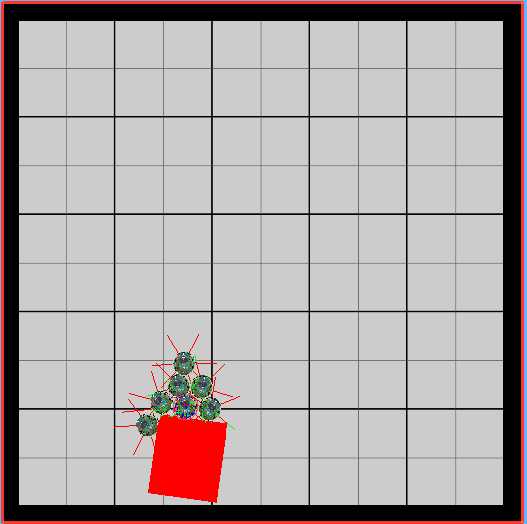
\includegraphics[scale=0.5]{figs/observation1}
\caption{Her setter du inn bildetekst}
\label{fig:o1}
\end{figure}

Unexpectedly, the robots sometimes formed lines, pushing the box by having one robot push the box and the other robots pushing each other as seen in figure ~\ref{fig:o0}.

\begin{figure}[p]
\centering
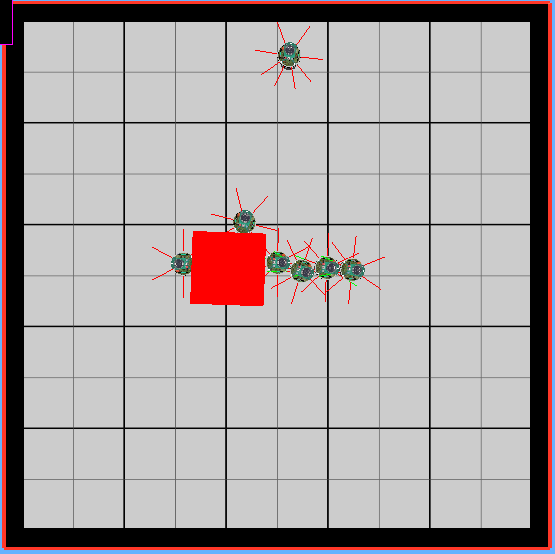
\includegraphics[scale=0.5]{figs/observation0.png}
\caption{The robots sometimes form long lines pushing each other}
\label{fig:o0}
\end{figure}

Robots never went into stagnation-mode while pushing the box and experimenting with the code led us to discover that this was due to how valuate\_pushing() is implemented and changed it slightly.
Robots would then often stagnate while successfully moving the box, one would think valuate\_pushing() prevented this behaviour and encouraged stagnation while the box is immobile.



\section{Suggestions for improving the design}

\subsection{Dynamic stagnation routine}
It quickly became apparant that our application would benefit from a more dynamic interval between pushing and evaluating the progress. Robots that were not positioned correctly would stay in an erronous position for just as many timesteps as a robot that was positioned correctly. We would propose to create a feedback system where the robots use observations from the environment to increase or decrease the amount of time it spends pushing before re-evaluating its position

\subsection{Rotation based search routine}
We observed that the robots were able to pick up the light from the food source from almost anywhere in the world. It would therefore be more beneficial for the search routine to revolve around more frequent rotation and less time going forward, as the robots would sometimes rotate away from the food source towards the outer perimiters and then proceed to distance itself from it.

\subsection{Distinguish between one and zero neighbours}
Robots that have one neighbour should be less likely to move than robots with zero, currently no distinction between the two.

%The stagnation-routine is too long
%Shorten the timed variables in stagnation, the movement pattern seems decent enough
%The search-routine should rotate around more, since the light-sensors can pick up the box from nearly everywhere in the world and aimlessly wandering wastes time. Often during stagnation the robot will just wander off towards the walls before returning.
%Robots should check if a robot is just behind them as well when they decide on whether to reposition or not, currently only checks to the left and right.
%Robots that were in a good position suddenly decide to move immediately after a neighbouring robot decides to leave, may want to run some timer that starts counting down when the robot realizes he is missing one of his two neighbours. Most commonly robots will gather in pairs of three only in one location, and even then the neighbours will eventually reposition themselves. Adding this timer will only serve to force the well positioned robots to stick around a little longer. Combined with shorter stagnation-routines there is a chance robots will return to their side
%Robots that have one neighbour should be less likely to move than robots with zero, currently no distinction between the two
%Propose to count all side- and back-sensors with higher values than 100 and add add to a percentage chance that these will move depending on number of 






\begin{figure}[p]
\centering
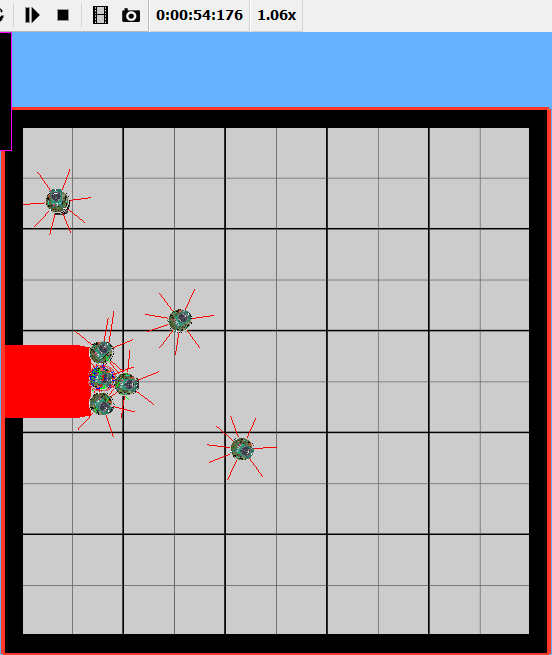
\includegraphics[scale=0.5]{figs/observation2}
\caption{Her setter du inn bildetekst}
\label{fig:02}
\end{figure}






\end{document}